\documentclass[12pt,a4paper]{article}

\usepackage[T1,T2A]{fontenc}
\usepackage[utf8]{inputenc}
\usepackage[russian]{babel}

%%%% Красная строка в русских текстах
\usepackage{indentfirst}

%%%% Настройка полей и отступов
\usepackage[a4paper,top=2cm,bottom=2cm,left=3cm,right=2cm,marginparwidth=1.75cm]{geometry}

%%%% Меняет стандартный формат нумерации секций
\usepackage{titlesec}
\titlelabel{\thetitle.\,\,}

%%%% Облегчают набор математических формул
\usepackage{amsmath}
\usepackage{amssymb}

%%%% Позволяют работать с графикой
\usepackage{graphicx}

%%%% Позволяет выделять текст цветом 
\usepackage{color}


\begin{document}

%%%%%%%%%%%%%%%%%%%%%%%%%%%
%%%%% ТИТУЛЬНЫЙ ЛИСТ %%%%%%
%%%%%%%%%%%%%%%%%%%%%%%%%%%
\begin{center} % включить выравнивание по центру
МИНИСТЕРСТВО ОБРАЗОВАНИЯ И НАУКИ РОССИЙСКОЙ \\
ФЕДЕРАЦИИ \\
Федеральное государственное автономное образовательное учреждение  \\
высшего образования\\ \textbf{<<Национальный исследовательский \\ Нижегородский государственный университет \\
им. Н.И. Лобачевского (ННГУ)>>}\\[1.5cm]%[4.5cm]
\textbf{Институт информационных технологий, математики и механики}\\[5.5cm]
%\textbf{Кафедра: Теории управления и динамики систем\\(ТУДС)}\\[0.8cm]
%Направление подготовки: \textbf{<<Математика и механика>>}\\
%направленность: \textbf{<<Дифференциальные уравнения, динамические системы и оптимальное управление>>}\\[2.2cm]

 \textbf{\large ОТЧЕТ} \\ % название работы, затем отступ 0,6см
 по \textbf{лабораторной} работе \\[0.6cm]
 
 на тему:\\
  \textbf{\large <<Исследование динамики системы с двумя параметрами>>}\\[6.5cm]
 % тема работы, затем отступ 3,7см
\begin{flushright}
 \begin{minipage}{0.52\textwidth} % начало маленькой врезки в половину ширины текста
 \begin{flushleft} % выровнять её содержимое по левому краю
  \textbf{Выполнил:} \\
 студент группы 3822Б1ПМ2 Махнёв Р.Д. \\
  \textbf{Проверил:}\\
 преподаватель каф. ТУДС Гринес Е.А.\\
 \end{flushleft} % конец выравнивания по левому краю
 \end{minipage} % конец врезки
\end{flushright}
 \vfill % заполнить всё доступное ниже пространство

  Нижний Новгород \\
 2024

 \thispagestyle{empty} % не нумеровать страницу

\end{center}

%%%%%%%%%%%%%%%%%%%%%%%%%%%%%%%%%%%%%
%%%%%%%% ОГЛАВЛЕНИЕ %%%%%%%%%%%%%%%%%
%%%%%%%%%%%%%%%%%%%%%%%%%%%%%%%%%%%%%
\renewcommand{\contentsname}{Содержание}
\newpage
\tableofcontents


%%%%%%%%%%%%%%%%%%%%%%%%%%%%%%%%%%%%%
%%%%%%%%% ОСНОВНАЯ ЧАСТЬ РАБОТЫ %%%%%
%%%%%%%%%%%%%%%%%%%%%%%%%%%%%%%%%%%%%
\newpage
\section{Анализ состояний равновесия системы}
Рассмотрим систему 
$$ 
\left \lbrace 
\begin{matrix}
\dot{x} = -x(b-x-y), \\
\dot{y} = (a-y)(2x+y).
\end{matrix} 
\right . .$$
Это нелинейная динамическая система, зависящая от параметров. Покажем, как построить для неё бифуркационную диаграмму.

% \subsection{Найти координаты всех состояний равновесия в зависимости от параметров}
Сначала найдём координаты всех присутствующих в ней состоянияй равновесия в зависимости от параметров.
Состояния равновесия находятся как решения системы уравнений 
$$ 
\left \lbrace 
\begin{matrix}
-x(b-x-y) =  0 \\
(a-y)(2x+y)  =  0
\end{matrix} 
\right . .$$
В результате получаем четыре состояния равновесия: $(0, 0)$, $(0, a)$, $( b-a , a)$ и 
$ ( -b, 2b) $.

%\subsection{Анализ матриц Якоби, поиск бифуркационных значений параметров}
Теперь найдём матрицу Якоби этой системы. Следуя стандартным обозначениям, примем $P(x, y) = -x(b-x-y)$ и $Q(x, y) = (a-y)(2x+y)$.
Вычислим частные производные:
$$ P'_x (x, y) = \frac{\partial}{\partial x}(-x(b-x-y)) = \frac{\partial (-x)}{\partial x} \cdot (b-x-y) - x \cdot \frac{\partial (b-x-y)}{\partial x} = 2x + y -b, $$
$$ P'_y (x, y) = \frac{\partial}{\partial y}(-x(b-x-y)) = \frac{\partial (-x)}{\partial y} \cdot (a-2x+3y) - x \cdot \frac{\partial(b-x-y)}{\partial y} = x, $$
$$ Q'_x (x, y) = \frac{\partial}{\partial x}((a-y)(2x+y)) = \frac{\partial (a-y)}{\partial x} \cdot (2x+y) + (a-y) \cdot \frac{\partial(2x+y)}{\partial x} = 2(a-y) = 2a-2y,$$
$$ Q'_y (x, y) = \frac{\partial}{\partial y}((a-y)(2x+y)) = \frac{\partial (a-y)}{\partial y} \cdot (2x+y) + (a-y) \cdot \frac{\partial(2x+y)}{\partial y} = a-2x-2y.$$

Подставим теперь координаты состояний равновесия и проанализируем собственные числа матриц Якоби. Матрица Якоби состояния равновесия равновесия $(0, 0)$ равна 
$$ \begin{pmatrix}
-b & 0 \\
2a & a 
\end{pmatrix} .$$
Матрица нижнетреугольная, а значит её собственные числа совпадают с её диагональными элементами:
$\lambda_1 = -b, \; \lambda_2 = a$. 
Собственные числа всегда вещественные, поэтому состояние равновесия может быть негрубым только когда одно из этих собственных чисел равно нулю. {\color{blue} Таким образом, бифуркационное множество для этого состояния равновесия -- $a = 0$ или $ b = 0$.} Опять же, так как мы явно знаем собственные числа матрицы Якоби, мы можем проанализировать тип состояния равновесия при любых значениях параметров: 
\begin{itemize}
	\item{$-b > 0, \; a > 0$ -- неустойчивый узел;}
	\item{$-b < 0, \; a < 0$ -- устойчивый узел;}
	\item{$-b > 0, \; a < 0$ или $-b < 0, \; a > 0$ -- седло.}
\end{itemize} 


Для состояния равновесия с координатами $(0, a)$ матрица Якоби равна
$$ \begin{pmatrix}
	a-b & 0 \\
	0 & -a 
\end{pmatrix} .$$

Матрица диагональная, а значит её собственные числа совпадают с её диагональными элементами:
$\lambda_1 = a-b, \; \lambda_2 = -a$. 
Собственные числа всегда вещественные, поэтому состояние равновесия может быть негрубым только когда одно из этих собственных чисел равно нулю. {\color{blue} Таким образом, бифуркационное множество для этого состояния равновесия -- $a = b$ или $ a = 0$.} 
Так как мы явно знаем собственные числа матрицы Якоби, мы можем проанализировать тип состояния равновесия при любых значениях параметров:  
\begin{itemize}
	\item{$a-b > 0, \; -a > 0$ -- неустойчивый узел;}
	\item{$a-b < 0, \; -a < 0$ -- устойчивый узел;}
	\item{$a-b > 0, \; -a < 0$ или $a-b < 0, \; -a > 0$ -- седло.}
\end{itemize}



Матрица Якоби, вычисленная в состоянии равновесия $\left ( b-a , a \right )$, равна   
$$ \begin{pmatrix}
	b-a & b-a \\
	0 & a-2b
\end{pmatrix} .$$
Матрица верхнетреугольная, а значит её собственные числа совпадают с её диагональными элементами:
$\lambda_1 = b-a, \; \lambda_2 = a-2b$. 
Собственные числа всегда вещественные, поэтому состояние равновесия может быть негрубым только когда одно из этих собственных чисел равно нулю. {\color{blue} Таким образом, бифуркационное множество для этого состояния равновесия -- $a = b$ или $ a = 2b$.} Поскольку здесь мы также явно знаем собственные числа матрицы Якоби, то мы можем проанализировать тип состояния равновесия при любых значениях параметров: 
\begin{itemize}
	\item{$b-a > 0, \; a-2b > 0$ -- неустойчивый узел;}
	\item{$b-a < 0, \; a-2b < 0$ -- устойчивый узел;}
	\item{$b-a > 0, \; a-2b < 0$ или $b-a < 0, \; a-2b > 0$ -- седло.}
\end{itemize}


Наконец, матрица Якоби в состоянии равновесия с координатами $ \left ( -b, 2b \right ) $  равна 
$$ \begin{pmatrix}
	-b & -b \\
	2a-4b &  a-2b
\end{pmatrix} .$$
Она не имеет какой-либо удобной структуры, поэтому для её исследования нужно исследовать её определитель и след:
$$ {\rm tr}\, J = a-3b $$
$$ {\rm det}\, J = 
-b \cdot (a-2b) + b \cdot (2a-4b) = 
b \cdot ( 2a-4b - (a-2b))  = b \cdot \left ( a-2b) \right. $$
Сначала проанализируем первое вырождение состояния равновесия, а именно -- наличие как минимум одного нулевого собственного число. 
Для этого определитель должен обратиться в ноль: 
$$ {\rm det}\, J = b \cdot \left ( a-2b) = 0\right.$$
Это уравнение имеет решения
$$
\left \lbrack 
\begin{matrix}
	b = 0 \\
	a = 2b
\end{matrix}
\right . .
$$
Проверим, имеет ли место второе вырождение 
$$ {\rm tr}\, J = 0, \; {\rm det}\, J > 0.$$
Для этого сначала решим уравнение ${\rm tr}\, J = 0$:
$${\rm tr}\, J = a-3b = 0,$$
откуда $a = 3b$.
Подставим теперь это в выражение для определителя.
Получим 
$$  b \cdot  ( a-2b) = b \cdot  ( 3b-2b) = b \cdot  b = b^2 \geq 0.$$
Таким образом, при $a = 3b, b \neq 0$ происходит второе вырождение, при котором у матрицы Якоби состояния равновесия появляется пара чисто мнимых собственных
чисел.
{\color{blue} Результирующее бифуркационное множество есть $b \cdot ( a-2b)=0$ или $a = 3b $ (при $b \ne 0 $).} С помощью следа и определителя мы можем определить, при каких значениях параметров данное состояние равновесия имеет определённый тип:
\begin{itemize}
	\item{$b \cdot ( a-2b) < 0$ -- седло (${\rm det}\, J < 0$); }
	\item{$b \cdot ( a-2b) > 0, \; a-3b > 0$ -- неустойчивый узел/фокус (${\rm det}\, J > 0, \; {\rm tr}\, J > 0$);}
	\item{$b \cdot ( a-2b) > 0, \; a-3b < 0$ -- устойчивый узел/фокус (${\rm det}\, J > 0, \; {\rm tr}\, J < 0$).}
\end{itemize} 


\subsection{Общая бифуркационная диаграмма для всех состояний равновесия}
Выпишем бифуркационное множество для всех состояний равновесия: 
\begin{itemize}
\item{$a = 0$ или $ b = 0$ для $(0, 0)$;}
\item{$a = b$ или $ a = 0$ для $(0, a)$;}
\item{$a = b$ или $ a = 2b$ для $\left (b-a , a \right )$;}
\item{$b = 0$ или $(a-2b)=0$ или $a = 3b $ (при $b \ne 0 $)  для $ \left ( -b, 2b  \right ) $.}
\end{itemize}
Воспользуемся GeoGebra для построения бифуркационного множества (по оси $x$ параметр $a$, а по оси $y$ -- параметр $b$).
\begin{figure}[!thb]
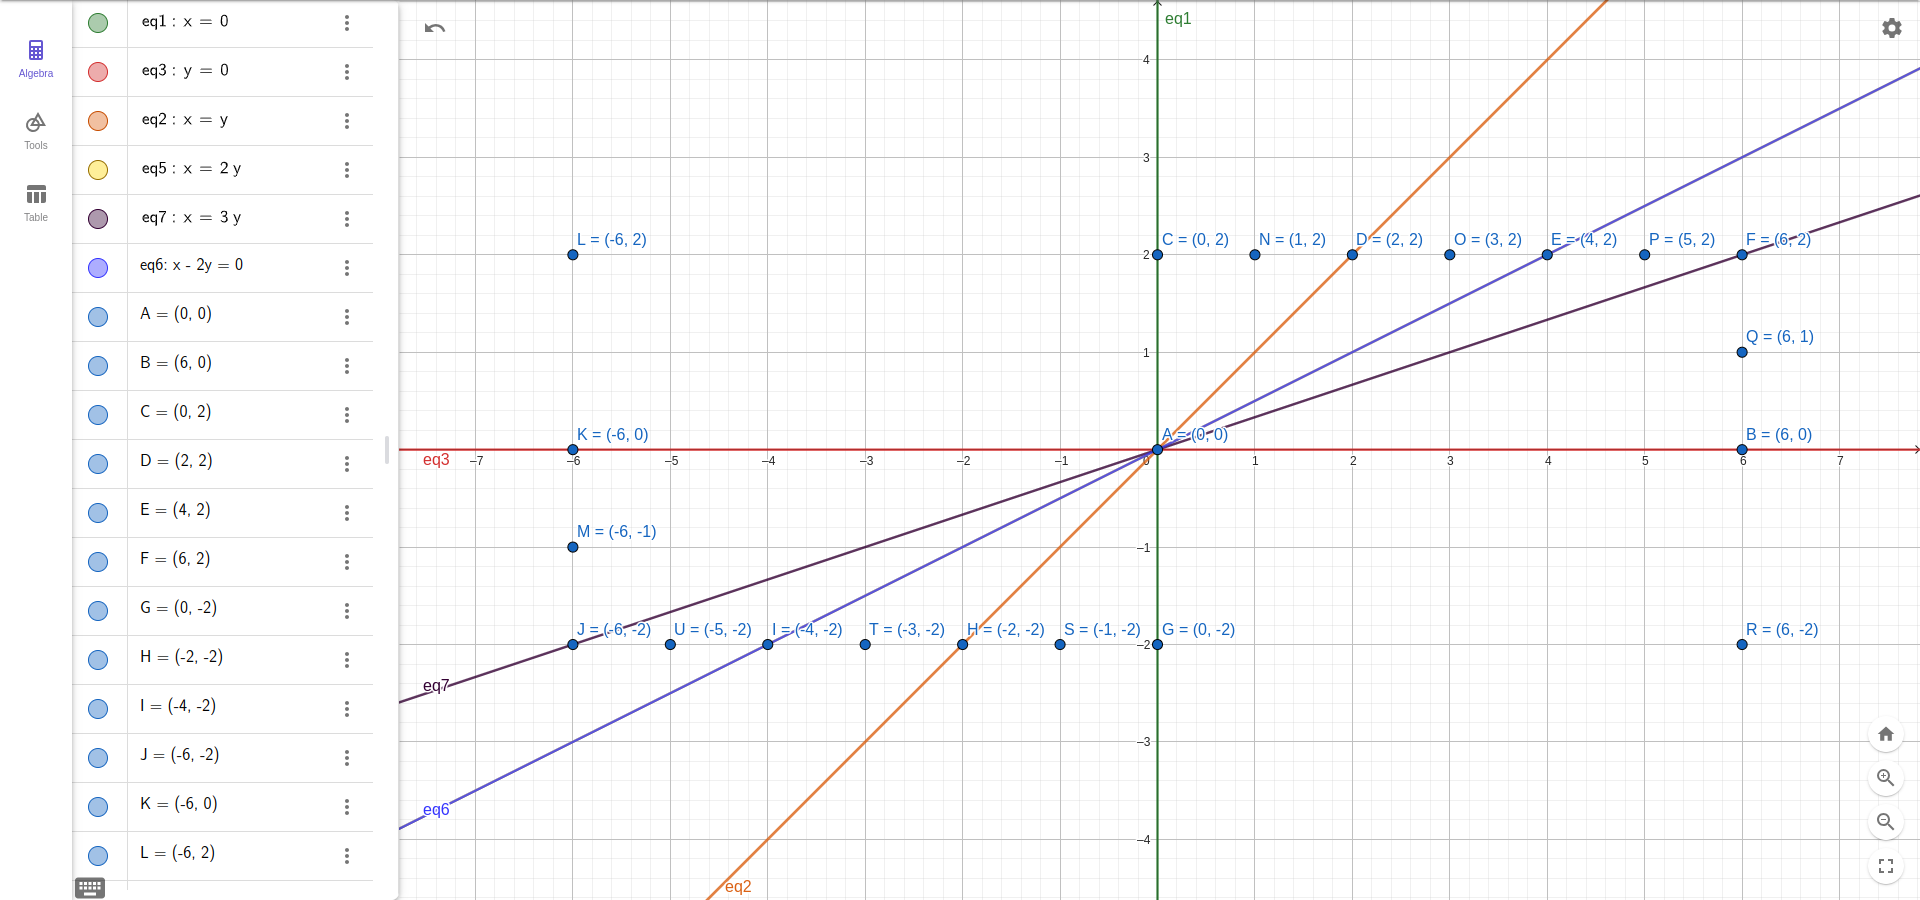
\includegraphics[height=8cm]{bifdiag-4.png}
\centering
\caption{\label{fig:bifdiag2} Бифуркационные границы данной системы.}
\end{figure}
Также отметим значения параметров, в которых будем определять типы состояний равновесия и строить фазовые портреты системы(см. рис. 1).



\newpage
\newpage

\subsection{Поиск инвариантных прямых}
Возьмем решение $(0, a)$ данной системы и выразим $y$ через $x$: $y = 0x+a$

Запишем и проверим, выполняется ли необходимое и достаточное условие инвариантности прямой $y = 0x+a$. 


\begin{center}
$Q(x, 0x+a) = 0 \cdot P(x, 0x+a)$

$0 \cdot (2x +a) = 0 \cdot  x(b - x - a)$
\end{center}
$0 = 0 \Rightarrow$ прямая $y = a$ является инвариантной прямой.

Теперь выразим $x$ через $y$: $x = 0y + 0$

Запишем и проверим, выполняется ли необходимое и достаточное условие инвариантности прямой $x = 0y + 0$
\begin{center}
$P(0, y) = 0 \cdot  Q(0, y)$

$0 \cdot (b - y) = 0 \cdot   y(a -y)$
\end{center}
$0 = 0 \Rightarrow$ прямая $x = 0$ является инвариантной прямой.


$$ 
\left \lbrace 
\begin{matrix}
-x(b-x-y) =  0 \\
(a-y)(2x+y)  =  0
\end{matrix} 
\right . .$$
\newpage
\section{Фазовые портреты системы}
\begin{enumerate} 
\item 
Возьмем следующие значения параметров:  $a^\ast = -4,\; b^\ast = 4$. При этих параметрах система будет иметь следующий вид:

$$ 
\left \lbrace 
\begin{matrix}
\dot{x} = -x(b-x-y), \\
\dot{y} = (a-y)(2x+y).
\end{matrix} 
\right . .$$

Состояния равновесия данной системы с выбранными параметрами: 
Определить тип каждого состояния равновесия можно двумя способами.
Во-первых, с помощью GeoGebra можно построить любое сочетание неравенств, которые определяют тип состояний равновесия.
Во-вторых, это можно сделать, взяв какие-нибудь конкретные значения параметров и проверив, какому из неравенств удовлетворяют значения параметров. 
Возьмем, например, $a^\ast = -4,\; b^\ast = 4$. 
Пересмотрим наши записи для каждого состояния равновесия: 
\begin{itemize}
\item{так как $-b^\ast < 0$ и $a^\ast < 0$, то $(0, 0)$ -- устойчивый узел;}
\item{так как $a^\ast -b^\ast < 0, \; -a^\ast > 0$, то $(0, a^\ast)$ -- седло; }
\item{так как $b^\ast-a^\ast > 0, \; a^\ast - 2b^\ast < 0$ , то $\left ( b^\ast-a^\ast , a^\ast \right )$ -- седло;}
\item{так как $b^\ast(a^\ast - 2 b^\ast) < 0$, то $  ( -b^\ast, 2b^\ast ) $ -- седло.}
\end{itemize}

\item
Возьмем следующие значения параметров:  $a^\ast = 1,\; b^\ast = 2$. При этих параметрах система будет иметь следующий вид: 

$$
\left \lbrace 
\begin{matrix} 
\dot{x} = -x \cdot (-x - y + 2), \\
\dot{y} = (1 - y) \cdot (2 \cdot x + y), \
\end{matrix} 
\right . .$$

Состояния равновесия данной системы с выбранными параметрами: $(0, 0)$, $(0, 1)$, $(-2, 4)$, $(1, 1)$. Определим тип каждого состояния равновесия, проверив, какому из неравенств удовлетворяют взятые значения параметров.  Пересмотрим наши записи для каждого состояния равновесия: 
\begin{itemize}
\item{ так как $-b^\ast  < 0 $ и $a^\ast > 0 $ то $(0, 0)$ -- Седло.}
\item{ так как $a^\ast - b^\ast  < 0 $ и $-a^\ast  < 0 $ то $(0, 1)$ -- Устойчивый узел.}
\item{ так как ${\lambda_{0}} > 0 $ и ${\lambda_{1}}  < 0 $ то $(-2, 4)$ -- Седло.}
\item{ так как $-a^\ast + b^\ast > 0 $ и $a^\ast - 2*b^\ast  < 0 $ то $(1, 1)$ -- Седло;}
\end{itemize} 

Возьмем следующие значения параметров:  $a^\ast = 1,\; b^\ast = 2$. При этих параметрах система будет иметь следующий вид: 

$$
\left \lbrace 
\begin{matrix} 
\dot{x} = -x \cdot (-x - y + 2), \\
\dot{y} = (1 - y) \cdot (2 \cdot x + y), \
\end{matrix} 
\right . .$$
+++++++++
Состояния равновесия данной системы с выбранными параметрами: $(0, 0)$, $(0, 1)$, $(-2, 4)$, $(1, 1)$. Определим тип каждого состояния равновесия, проверив, какому из неравенств удовлетворяют взятые значения параметров.  Пересмотрим наши записи для каждого состояния равновесия: 
\begin{itemize}
\item{ так как $-b^\ast  < 0 $ и $a^\ast > 0 $ то $(0, 0)$ -- Седло.}
\item{ так как $a^\ast - b^\ast  < 0 $ и $-a^\ast  < 0 $ то $(0, 1)$ -- Устойчивый узел.}
\item{ так как ${\lambda_{0}} > 0 $ и ${\lambda_{1}}  < 0 $ то $(-2, 4)$ -- Седло.}
\item{ так как $-a^\ast + b^\ast > 0 $ и $a^\ast - 2*b^\ast  < 0 $ то $(1, 1)$ -- Седло;}
\end{itemize} 


Возьмем следующие значения параметров:  $a^\ast = 1,\; b^\ast = 5$. При этих параметрах система будет иметь следующий вид: 

$$
\left \lbrace 
\begin{matrix} 
\dot{x} = -x \cdot (-x - y + 5), \\
\dot{y} = (1 - y) \cdot (2 \cdot x + y), \
\end{matrix} 
\right . .$$

\newpage

Возьмем следующие значения параметров:  $a^\ast = 1,\; b^\ast = 5$. При этих параметрах система будет иметь следующий вид: 

$$
\left \lbrace 
\begin{matrix} 
\dot{x} = -x \cdot (-x - y + 5), \\
\dot{y} = (1 - y) \cdot (2 \cdot x + y). \
\end{matrix} 
\right . .$$

Состояния равновесия данной системы с выбранными параметрами: $(0, 0)$, $(0, 1)$, $(-5, 10)$, $(4, 1)$. Определим тип каждого состояния равновесия, проверив, какому из неравенств удовлетворяют взятые значения параметров.  Пересмотрим наши записи для каждого состояния равновесия: 
\begin{itemize}
\item{ так как $-b^\ast  < 0 $ и $a^\ast > 0 $ то $(0, 0)$ -- седло;}
\item{ так как $a^\ast - b^\ast  < 0 $ и $-a^\ast  < 0 $ то $(0, 1)$ -- устойчивый узел;}
\item{ так как ${\lambda_{1}} = - \sqrt{94} - 7  < 0 $ и ${\lambda_{2}} = -7 + \sqrt{94} > 0 $ то $(-5, 10)$ -- седло;}
\item{ так как $-a^\ast + b^\ast > 0 $ и $a^\ast - 2*b^\ast  < 0 $ то $(4, 1)$ -- седло.}
\end{itemize} 


\end{enumerate}
\end{document}
